\documentclass[sutton_barto_notes.tex]{subfiles}

\begin{document}

\newpage
\section{Chap. 2 Multi-armed Bandits}
\begin{itemize}
\item Evaluative: feedback depends solely on the taken action, indicating results
\item Instructive: feedback is independent of the taken action, indicating correct actions
\item Nonassociative setting: no learning involved in more than one situation; no need to associate different actions with different situations/states
\item Associative setting: the best action depends on the situation
\end{itemize}

\begin{figure}[!h]
  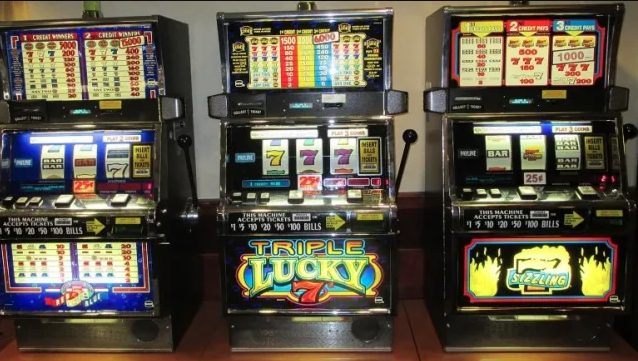
\includegraphics[width=\linewidth]{one-armed-bandit.png}
  \caption{Three one-armed/level bandit machines}
  \label{fig:bandit-machine}
\end{figure}

\subsection{A k-armed Bandit Problem}

\textit{k-armed bandit problem}:
You choose one action from \textit{k} available actions (e.g. choose one of the slot machines). For each choice, you receive a numerical reward. The reward is given based on a probability distribution that specific to the choice (machine). Your objective is to maximize the expected total reward over \textit{j} action selections (time steps).

Note that the bandit problem is formally equivalent to a one-state Markov decision process. 

For now, let us define that
\begin{itemize}
\item \textit{Value}: the expected/mean reward of a taken action
\item $A_t$: action selected on time step $t$
\item $R_t$: corresponding reward of $A_t$
\item $q_{*}(a)$:  $q_{*}(a) \doteq \E[R_t|A_t=a]$. The (true) value of an arbitrary action $a$ (i.e. the expected reward given $a$ is selected)
\item $Q_t(a)$: the \textit{estimated} value of action $a$ at time step $t$.
\end{itemize}

If we know each action values, then solving the \textit{k}-armed bandit problem would be always select the action with highest $value$.
If we don't know the action values, then we can estimate them.
Our goal is to have $Q_t(a)$ to be as close to $q_*(a)$ as possible.

\begin{definition}
\textbf{Greedy actions}, action(s) with highest \textbf{estimated} value.
\end{definition}
\textit{exploiting}: select greedy action(s).
\textit{exploring}: select non-greedy action(s). Exploration may improve the estimate value of non-greedy actions.

\subsection{Action-value Methods}

\begin{definition}
\textbf{Action-value Methods}, or Q function, methods for estimating the values of actions, and using the estimates to select actions.
\end{definition}

`Q' means the \textbf{quality} of an action.

Let see a simple action-value method: \textit{sample-average method}, in which action-value is the mean reward for an action.

$$ Q_t(a) \doteq \frac{\sum_{i=1}^{t-1}R_i \cdot \1_{A_{i=a}}}{\sum_{i=1}^{t-1}\1_{A_{i=a}}}$$

\begin{itemize}
	\item $\1$: return 1 if predicate is true, otherwise 0
	\item in the case when denominator is 0 (which makes the fraction mathematically undefined), $Q_t(a)$ is set as default value (e.g. 0)
	\item in the case when denominator $\rightarrow \infty$, by the Law of Large Numbers, $Q_t(a)$ converges to $q_*(a)$
\end{itemize}

\begin{definition}
\textbf{Greedy action selection}, If there are more than one greedy action, select one of them arbitrarily.
$$ A_t \doteq \argmax_{a} Q_t(a) $$
\end{definition}

\begin{definition}
\textbf{$\varepsilon$-greedy action selection} with probability $\varepsilon$, select an action randomly; with probability $1-\varepsilon$, select a greedy action
\end{definition}

\subsection{The 10-armed Testbed}

For Exercise 2.2, note that we should first convert the sequence of actions and rewards to $Q_t(a)$, then we can decide whether the selection is greedy or exploration based on the definition of $\varepsilon$-greedy action selection.

\subsection{Incremental Implementation}

Recall that estimated action value $Q_n$, using sample-average method, is calculated as:
$$ Q_n \doteq \frac{R_1 + \cdots + R_{n-1}}{n-1} $$

We don't want to waste memory and computational resource for each new reward.
Intuitively, to save memory, we can simplify the equation by first reconstruct the previous estimated action value $Q_{n-1}$ and then evaluate $Q_n$ with the new reward $R_n$.
Therefore,
$$ Q_{n+1} = \frac{Q_n \cdot (n-1) + R_n}{n} = \frac{Q_n \cdot n - Q_n + R_n}{n} = Q_n + \frac{1}{n}[R_n - Q_n] $$

The form $Q_{n+1} = Q_n + \frac{1}{n}[R_n - Q_n]$ is an important form occurs in this book. The general form is
$$ NewEstimate \leftarrow OldEstiamt + StepSize\underbrace{[Target - OldEstimate]}_{error} $$

% \begin{tcolorbox}[width=\textwidth,colback={grey},title={A simple bandit algorithm},colbacktitle=black,coltitle=white]}
\begin{tcolorbox}[width=\textwidth,title={A simple bandit algorithm}]
	\begin{align*}
	   & \text{Initialize, for a = 1 to }k: \\
	   & \quad Q(a) \leftarrow 0 \\
	   & \quad N(a) \leftarrow 0 \\
	   & \text{Loop forever: }\\
	   & \quad A \leftarrow \left\{
	    \begin{array}{ll}
	        \argmax_x Q(a) & \text{with prob. } 1 - \varepsilon \text{ (breaking ties randomly) }\\
	        \text{a random action} & \text{with prob. } \varepsilon
	    \end{array}
	\right. \\
	   & \quad R \leftarrow bandit(A) \\
	   & \quad N(A) \leftarrow N(A) + 1 \\
	   & \quad Q(A) \leftarrow Q(A) + \frac{1}{N(A)}[R-Q(A)]
	\end{align*}
\end{tcolorbox}

\subsection{Tacking a Nonstationary Problem}

Rewrite the update equation from last section and replace the stepsize with $\alpha$, we have that

$$ Q_{n+1} = (1-\alpha)^n Q_1 + \sum_{i=1}^n \alpha (1-\alpha)^{n-i} R_i$$

The first term tells us that contribution of $Q_1$ decreases exponentially with time, and the second term tells us the older rewards contribute exponentially less to the sum; i.e., the most recent rewards contribute most to our current estimate.

In previous section, the reward probability distribution is stationary (i.e. doesn't change over time).
For nonstatoinary cases, let say we give more weight to recent rewards than to `long-past' rewards; for doing so, one popular way is to use a constant $\alpha$ (step size).

Not all choices of $\alpha_n(a)$ guarantee convergence.
In \textit{stochastic approximation theory}, two conditions required to assure convergence ``with probability 1''\footnote{i.e. \textit{almost sure}. No distinction between `sure' and `almost sure' in finite sample space, but becomes important in infinite sample space. see \url{https://en.wikipedia.org/wiki/Almost_surely}}:

$$ \sum_{n=1}^\infty \alpha_n(a) = \infty $$
$$ \sum_{n=1}^\infty \alpha_n^2(a) < \infty $$

The 1st condition is required to guarantee that the steps are large enough to eventually overcome any initial conditions or random fluctuations.
The 2nd condition is required to guarantee that the steps eventually become small enough to assure convergence.

Therefore, in sample-average method, $\alpha_n(a) = \frac{1}{n}$ converges, but a constant step-size parameter $\alpha_n(a)=\alpha$ does not converge.

Note that sequences of $\alpha$ that meet the conditions often converge very slowly and often need considerable tunning.
These sequences of $\alpha$ often used in theoretical work, and are seldom used in real-world application.

\subsection{Optimistic Initial Values}

Higher (optimistic) initial values ($Q_i(a)$) encourages more \textit{early} exploration. Because whichever actions are initially selected, the
reward is less than the starting estimates; the agent then switches to other actions. This encourages more explorations early on.

However, this may only work well on stationary problems; as in nonstationary problems, some action values may change after certain timesteps. Another limitation is that we may not know what the optimistic initial value should be. Though a combination of exploration technique may be adequate in practice.

\subsection{Upper-Confidence-Bound Action Selection}

In $\varepsilon$-greedy action selection, it is not ideal to just randomly select actions; instead, we want to select among the non-greedy actions according to their potential for actually being optimal. Such taking into account both (1) how close their estimates are to being maximal, and (2) the uncertainties in those estimates.

\begin{definition}
Upper-Confidence-Bound (UCB) Action Selection

\[
A_t \doteq \argmax_a \bigg[ \underbrace{Q_t(a)}_{\text{exploitation term}} + \underbrace{c\sqrt{\frac{\text{ln }t}{N_t(a)}}}_{\text{exploration term}} \bigg]
\]
\end{definition}
$N_t(a)$, denotes the number of times that action $a$ has been selected prior to time $t$. If $N_t(a)=0$, then $a$ is considered to be a maximizing action.
$c$, $c > 0$ (confidence level) controls the degree of exploration.

\begin{figure}[!h]
  \centering
  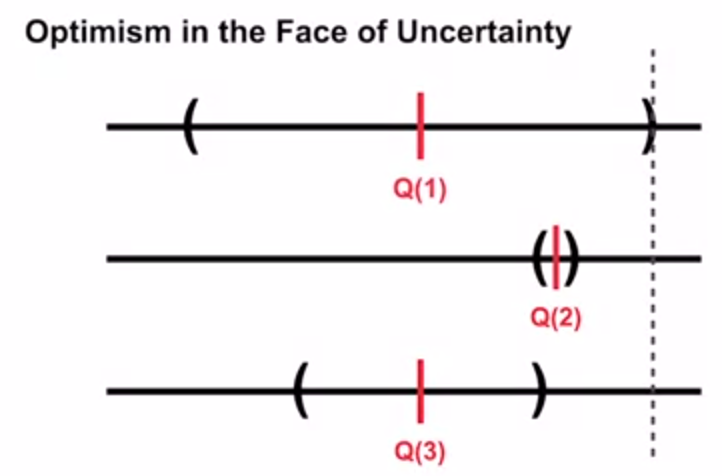
\includegraphics[width=0.7\linewidth]{UCB_example.png}
  \caption{UCB Example with 3 actions. The interval represents the confidence level of the action. Larger confidence, smaller interval. Given the 3 actions, we select the one with highest upper bound. We update the interval based on received rewards.}
  \label{fig:UCB_example}
\end{figure}

The idea of UCB action selection is that the square-root term is a measure of the uncertainty/variance in the estimate of $a$'s value.
Each time $a$ is selected, the uncertainty is (presumably) reduced as $N_t(a)$ increments.
Each time a non-$a$ is selected, $t$ increments but $N_t(a)$ doesn't, thus the uncertainty estimate increases.
All actions will eventually be selected, but actions with lower value estimates or that have been frequently selected, will be selected with decreasing frequency over time.

UCB is useful in bandit problems, but is (usually) not practical in general RL settings. It is difficult to deal with (1) nonstationary problems, and (2) large state spaces.

\subsection{Gradient Bandit Algorithms}
We have considered methods that (1) estimate actions values; (2) select actions based on estimations.
We now consider a new approach for action selection: learning a numerical \textit{preference} for each action \textit{a}, which we denote $H_t(a) \in \R$.
The larger the preference, the more often that action is taken, but the preference has no interpretation regarding rewards.
Only the \textbf{relative} preference of one action over another is important.
The action probabilities is determined by \textit{soft-max distribution}.

\[
P(A_t=a) \doteq \frac{e^{H_t(a)}}{\sum_{b=1}^k e^{H_t(b)}} \doteq \pi_t(a)
\]

$\pi_t(a)$ is the probability of taking action $a$ at time $t$. The initial probability are the same for all actions.

There is a natural learning algorithm in this setting based on the idea of stochastic gradient descent.
This is based on updating the preference values as such, after taking action $A_t$ and obtaining reward $R_t$

$$ H_{t+1}(A_t)\doteq H_t(A_t) + \alpha (R_t - \overline{R_t})(1-\pi_t(A_t)) $$

$$ H_{t+1}(a) \doteq H_t(a) - \alpha(R_t - \overline{R_t})\pi_t(a)\quad\text{for all }a\neq sA_t $$

$\overline{R_t} \in \R $ is the average of the rewards up to but not including time $t$ (with $\overline{R_1} = R_1$)

If the reward is higher than the baseline $\overline{R_t}$, then the probability of taking $A_t$ in the future is increased; and if the reward is below baseline, then the probability is decreased.
The non-selected actions move in the opposite direction.

The above update scheme is equivalent to \textbf{stochastic gradient ascent} with batch size 1.

\subsection{Associative Search (Contextual Bandits)}

For now, we have only considered nonassociative tasks, that is, tasks in which there is no need to associate different actions with different situations.
However, in the general RL task, there is more than one situation/state, and the goal is to learn a policy, i.e., a mapping from states to optimal actions given the state.

Suppose when a bandit task is selected for you, you are given some distinctive clue about its identity (but not its action values). For instance, if screen=red (actual reward is hidden from you), select arm 1; if screen=green, select arm 2... This is an example of an associative search task, it involves both trial-and-error learning to search for the best actions, and association of these actions with the situations in which they are best. This task is now called \textit{contextual bandits} in the literature.

In this setting, we still don't have actions affecting the next situation as well as the reward. This will add another layer of complexity and lead us to full RL problems.

\begin{itemize}
\item (level 1) $k$-armed bandit problem: select one of $k$ actions that have fixed probabilities. For each selected action, a reward is given. The goal is to maximize the total reward after $j$ selections.
\item (level 2) associative search task (contextual bandits): Same as $k$-armed bandit problem, the action affects only the immediate reward. Unlike $k$-armed bandits problem, what situations/state you are facing are told and it involves learning a policy.
\item (level 3) full RL problem: On top of associative search task, actions affect next situation and reward.
\end{itemize}

\subsection{Summary}

This chapter presented several ways to balance exploration and exploitation:

\begin{itemize}
\item $\varepsilon$-greedy methods choose randomly among actions a small fraction of the time to encourage exploration
\item UCB methods choose deterministically but favouring actions with uncertain estimates
\item Gradient methods don't estimate action values, but preferences, and choose actions probabilistically according to the preferences
\item Optimistic initialization sets optimistic initial $Q$ values in order to encourage a very active exploration in the initial phase, leading to a fast convergence with no bias
\end{itemize}

There is no method among the above that is best. Common ways to assess performance of these kind of algorithms are through graphs:
\begin{itemize}
\item learning curve: shows the performance of an algorithm vs. iterations for a certain parameter setting
\item parameter studies: summarize each algorithm by the average reward over the first 1000 steps, and show such a value for various parameter settings and algorithms.
\end{itemize}

One should also consider the sensitivity to parameter setting, that is an indication of \textbf{robustness}.

Despite the simplicity of methods presented in this chapter, they can be considered state of the art. More sophisticated methods usually impose additional complexity and assumptions.

Another approach to balancing exploration and exploitation in $k$-armed bandit problems is to compute a special kind of action value called \textit{Gittins index}, which is an instance of Bayesian methods. This assume a known initial distribution over the (stationary) action values and then update the distribution exactly after each step.
In general, the update computations are complex, but for \textit{conjugate priors} they are easy.
One way to select the best action at each time step is based on posterior probability.
This method, sometimes called posterior sampling or Thompson sampling.

\newpage
\subsection{Learning Objectives (UA RL MOOC)}

Lesson 1: The K-Armed Bandit Problem

1. Define reward

A number received for each taken action.

2. Understand the temporal nature of the bandit problem

Temporal means "related to time" in RL. From my understanding, the temporal nature of the bandit problem is that the decision of choosing action depends on which time steps in.
For instance, on time step one, when the gambler does not have knowledge of the "value" of each machine, he needs to play a machine randomly. On time step two, he may play a different machine than on step one. After some rounds, the gambler has some value estimations of each machine; he then can play greedily with the highest value action.
In general, the action selection strategy hinges on time steps, i.e., the action selection is temporal dependent.

3. Define k-armed bandit

Given k actions/choice, each with a numerical reward, each reward are given based on fixed probabilities. You need to do this selection in multiple rounds and your aim is to maximize the total reward.

4. Define action-values

values = action values = action value function

Action-value is the mean/expected reward of an action.


Lesson 2: What to Learn? Estimating Action Values

1. Define action-value estimation methods

$$Q(a) = \frac{\sum R}{\text{action count}}$$

2. Define exploration and exploitation

Exploration select random actions and exploitation select greedy action.

3. Select actions greedily using an action-value function

$$A = argmax(q_values)$$

4. Define online learning

Online learning is when the agent interacts with the environment.
Offline learning is when the agent learns from fixed datasets

5. Understand a simple online sample-average action-value estimation method

$$Q_{n+1} = Q_n + \frac{1}{n}[R_n - Q_n]$$

6. Define the general online update equation

$$Q_{n+1} = Q_n + \frac{1}{n}[R_n - Q_n]$$

7. Understand why we might use a constant stepsize in the case of non-stationarity

Use a constant stepsize makes the agent able to adapt to changing environment.
If we use 1/N(a) as stepsize in non-stationary cases, when the true values change suddenly in long steps, the 1/N(a) may be very small and can hardly learn the new values.

Lesson 3: Exploration vs. Exploitation Tradeoff

8. Define epsilon-greedy

Epsilon-greedy is used to balance exploitation and exploration. With small probability epsilon, we choose randomly among all actions (exploration), with 1-epsilon probability, we choose the highest value action (exploitation).

9. Compare the short-term benefits of exploitation and the long-term benefits of exploration

The short-term benefits of exploitation is we maximize the reward immediately, the long-term benefits of exploration is we have a better knowledge of the estimated values (i.e., Q(a)->q*(a)), thus giving us higher total rewards in the long run.

10. Understand optimistic initial values

We declare initial values way higher than their true values, thus the name optimistic. In such way, we are encouraged to try out all actions early on. When one action is selected, its value is certainly to drop (since we assign high initial value), allowing other non-touched actions to be selected.

11. Describe the benefits of optimistic initial values for early exploration

see 10

12. Explain the criticisms of optimistic initial values

Optimistic initial values may only well on stationary cases. In nonstationary cases, the advantage of optimistic dwindles as the step size increases.
Another disadvantage is that we do not know how to select the "correct" optimistic initial values.

13. Describe the upper confidence bound action selection method

This is also a exploration-exploitation balancing technique. This encourages the agent to choose the action with highest UCB. The more an action is selected, the narrower the confidence interval of an action is, the less the explore-term of the action is.

14. Define optimism in the face of uncertainty

We always select the action with highest (most optimistic) UCB. When the action is selected, it either be good (the UCB largely stays) or bad (the UCB shrinks and enable other actions to be selected).


15. Different constant step size and decaying step size

A larger step size moves us more quickly toward the true value, but can make our estimated values oscillate around the expected value. A step size that reduces over time can converge to close to the expected value, without oscillating. On the other hand, such a decaying stepsize is not able to adapt to changes in the environment. Nonstationarity---and the related concept of partial observability---is a common feature of reinforcement learning problems and when learning online


\end{document}